\documentclass[a4paper,9pt]{article}
\usepackage[margin=1.55cm]{geometry}
\usepackage{amsmath,amssymb,booktabs,graphicx,hyperref,microtype}
\usepackage[T1]{fontenc}
\usepackage[utf8]{inputenc}
\hypersetup{colorlinks=true,linkcolor=black,urlcolor=blue,citecolor=black}
\setlength{\parskip}{0.25em}\setlength{\parindent}{0pt}
\newcommand{\teamname}{lifeisluck}
\newcommand{\contactemail}{kimbumjun001027@gmail.com}
\title{\vspace{-1.1cm}\large PERPETUAL ALPHA 2026\\[1.5mm]Technical Report}
\author{\teamname{} \;|\; \texttt{\contactemail}}\date{6 November 2026}
\begin{document}\maketitle\vspace{-0.6cm}
\begin{abstract}
We implement a fixed, hourly pair-reversion strategy for PAS DEX on Hyperliquid
Testnet. It trades beta-adjusted return gaps in BTC--EWY and BTC--ETH subject to
correlation, volatility, exposure, and account-level loss gates. Parameters
were selected using chronological historical segments and were not retrained
during the live phase. This report states the live record and its limitations.
\end{abstract}

\section{Strategy overview}
The agent is a relative-value strategy, not a directional forecaster. It enters
only after a correlated BTC--$B$ pair develops a beta-adjusted return gap,
shorting the relative outperformer and buying the underperformer. Both legs use
equal USD notionals. Pair risk is allocated 85\% to BTC--EWY and 15\% to
BTC--ETH; decisions use completed hourly candles only.

This construction separates pair selection from trading direction. Pair
selection asks whether a relationship has been sufficiently stable to make a
relative-value trade meaningful; the gap sign then determines which leg is long
and which is short. The agent does not predict the next BTC, ETH, or EWY price
in isolation. It instead requires evidence of co-movement first and takes a
position only when the relationship deviates beyond a common threshold.

\section{Methodology and models}
Let $r_t^B$ and $r_t^{BTC}$ be hourly log returns. For a rolling window $W$,
\[
\beta_t=\frac{\operatorname{Cov}_W(r^B,r^{BTC})}{\operatorname{Var}_W(r^{BTC})},\qquad
g_t=\log\left(\frac{P_t^B}{P_{t-L}^B}\right)-\beta_t\log\left(\frac{P_t^{BTC}}{P_{t-L}^{BTC}}\right).
\]
Entry requires rolling correlation $\geq0.70$ and $|g_t|\geq1.5\%$.
BTC--EWY uses $W=24$, $L=12$ hours; BTC--ETH uses $W=72$, $L=3$.
The beta adjusts the signal; equal-dollar legs are deliberately used for
execution simplicity, so this is not a fully beta-neutral hedge.

Organizer-provided hourly BTC, ETH, and EWY history was split chronologically
into train, validation, and final-test segments. A small allocation/exposure
grid was compared with a score proxy. Faster variants, simple stop-loss
overlays, and extra pairs were rejected when post-cost or later-segment evidence
was not robust.

The validation sequence was deliberately chronological: parameter alternatives
were screened on the first segment, compared on a later validation segment, and
then checked once more on a final holdout segment. We did not shuffle time
series observations or repeatedly tune the final holdout. The score proxy
included the competition's return-volatility trade-off, rather than selecting a
configuration only on raw cumulative return. This is why a moderate gross
exposure and a two-pair portfolio were preferred to a concentrated or
high-turnover alternative.

\begin{table}[h]\centering\small
\caption{Chronological historical score-proxy comparison.}
\label{tab:allocation}
\begin{tabular}{lrrr}\toprule
Configuration & Train & Validation & Final test\\ \midrule
80\% EWY / 20\% ETH, 50\% gross & 0.1584 & 0.0902 & 0.1048\\
85\% EWY / 15\% ETH, 50\% gross & 0.1620 & 0.0994 & 0.1058\\
85\% EWY / 15\% ETH, 65\% gross & 0.1734 & 0.1033 & 0.1125\\ \bottomrule
\end{tabular}\end{table}

\begin{table}[h]\centering\small
\caption{Robustness screens used to keep the final rule set small.}
\begin{tabular}{p{3.2cm}p{5.7cm}}\toprule
Candidate & Decision and reason \\ \midrule
Sub-hourly / minute rules & Not adopted: later-window evidence did not remain positive after conservative costs. \\
Additional pairs (including ETH--HYPE) & Not adopted: did not improve the later chronological segment consistently. \\
Simple fixed stop-loss & Not adopted: reduced historical score-proxy performance without reliably avoiding widening regimes. \\
Beta-sized execution legs & Not adopted: lower-risk episodes were observed, but no stable return advantage versus equal-dollar legs. \\
\bottomrule\end{tabular}\end{table}

Table~\ref{tab:parameters} records why the final numerical settings were
retained. It distinguishes values selected from the chronological comparison
from deliberately simple risk guardrails. The latter were not tuned to maximize
historical return, because treating risk limits as another free parameter would
make the backtest appear more precise than the available sample supports.

\begin{table}[h]\centering\small
\caption{Parameter rationale and selection status.}
\label{tab:parameters}
\begin{tabular}{p{2.9cm}p{2.3cm}p{4.4cm}}\toprule
Parameter & Final value & Rationale \\ \midrule
Correlation gate & $\rho\geq0.70$ & Requires a materially positive relationship before interpreting a return gap as relative dislocation rather than two unrelated moves. Kept fixed after pair screening. \\
Entry gap & $|g|\geq1.5\%$ & Filters small moves that are more likely to be noise or consumed by round-trip costs. Selected from the small chronological signal screen, not re-tuned online. \\
Signal windows & EWY: $W/L=24/12$ h; ETH: $72/3$ h & Pair-specific windows were retained because they produced the strongest score-proxy result across later chronological segments within the tested set. \\
Portfolio allocation & EWY/ETH $=85/15$; gross $=65\%$ & Highest score proxy in each of train, validation, and final-test comparisons in Table~\ref{tab:allocation}; the gross cap also limits account-level volatility. \\
High-volatility scaler & 75\% size when BTC 24 h volatility $\geq0.6\%$ & A discrete, interpretable reduction during high-volatility conditions. It is a conservative guardrail, not a fitted return-maximizing parameter. \\
Exit rules & EWY: 12 h / full recovery; ETH: 24 h / 50\% recovery & Empirical holding bounds that allow reversion time while preventing stale exposure; adverse-widening rules provide an additional failure exit. \\
Loss gates & 3\% daily loss; 6\% peak drawdown & Non-optimized account-level circuit breakers. The daily gate prevents a single session from consuming the full peak-drawdown budget. \\
\bottomrule\end{tabular}\end{table}

\section{Data}
Research used organizer-provided hourly PAS history. The deployed agent reads
public PAS Testnet market and account data, aligned by completed hour. No paid
or proprietary external data are used; order-book data support execution checks,
not directional prediction.

For each decision time, the calculation uses only information available at the
close of the previous hourly candle. The engine computes rolling returns,
correlation, beta, and BTC realized volatility on the aligned series, evaluates
the entry and risk gates, and acts only at the next scheduled check. This
ordering avoids using an incomplete candle as if it were known at decision time.

\section{Risk management}
Gross exposure is capped at 65\% of account equity. New entries are scaled to
75\% when 24-hour BTC realized volatility is at least 0.6\%. The engine blocks
new entries after a 3\% daily loss or 6\% peak-to-trough drawdown and rejects
material leg mismatch.
BTC--EWY exits on full recovery, 100\% adverse widening, or 12 hours;
BTC--ETH exits on 50\% recovery, 50\% adverse widening, or 24 hours. Holding
limits are empirical risk caps, not theoretical proofs of convergence.

The exit hierarchy is important. Recovery exits monetize the relative gap when
the hypothesis works; adverse-widening and time exits keep a failed or stale
relationship from remaining open indefinitely. The model can still lose during
a persistent regime change, so these controls cap exposure duration rather than
claiming to eliminate tail risk.

The design targets the competition financial score
\[
Q=\frac{\max(R,0)+0.005}{|R|+1.5\sigma+0.05},
\]
where $R$ and $\sigma$ are the organizer-defined daily-snapshot return and
volatility.

\section{Execution and infrastructure}
The agent runs locally as a scheduled short process. Each invocation reads the
latest completed candle, persists state and an audit log, then exits. Orders are
restricted to Hyperliquid Testnet PAS and require wallet, state, position,
slippage, timeout, and leg-mismatch checks.

\section{Results and analysis}
Figure~\ref{fig:results} uses Hyperliquid Testnet's public portfolio PnL history
queried on 06 November 2026, 03:04 UTC. Latest observed platform PnL was USDP -2,830; maximum
drawdown from a prior PnL peak was USDP 2,830. These approximately 15-minute
platform observations are not the competition's 12:00 UTC daily snapshots and
must not be substituted for official leaderboard return or score. The record
shows the key risk: a few adverse widening episodes can dominate small recoveries.

This live path is therefore presented as operational evidence rather than a
fresh optimization target. The report does not modify the final parameters to
fit the observed drawdown, because doing so from a small number of live trades
would make the resulting model less credible and more prone to overfitting.

\begin{figure}[h]\centering
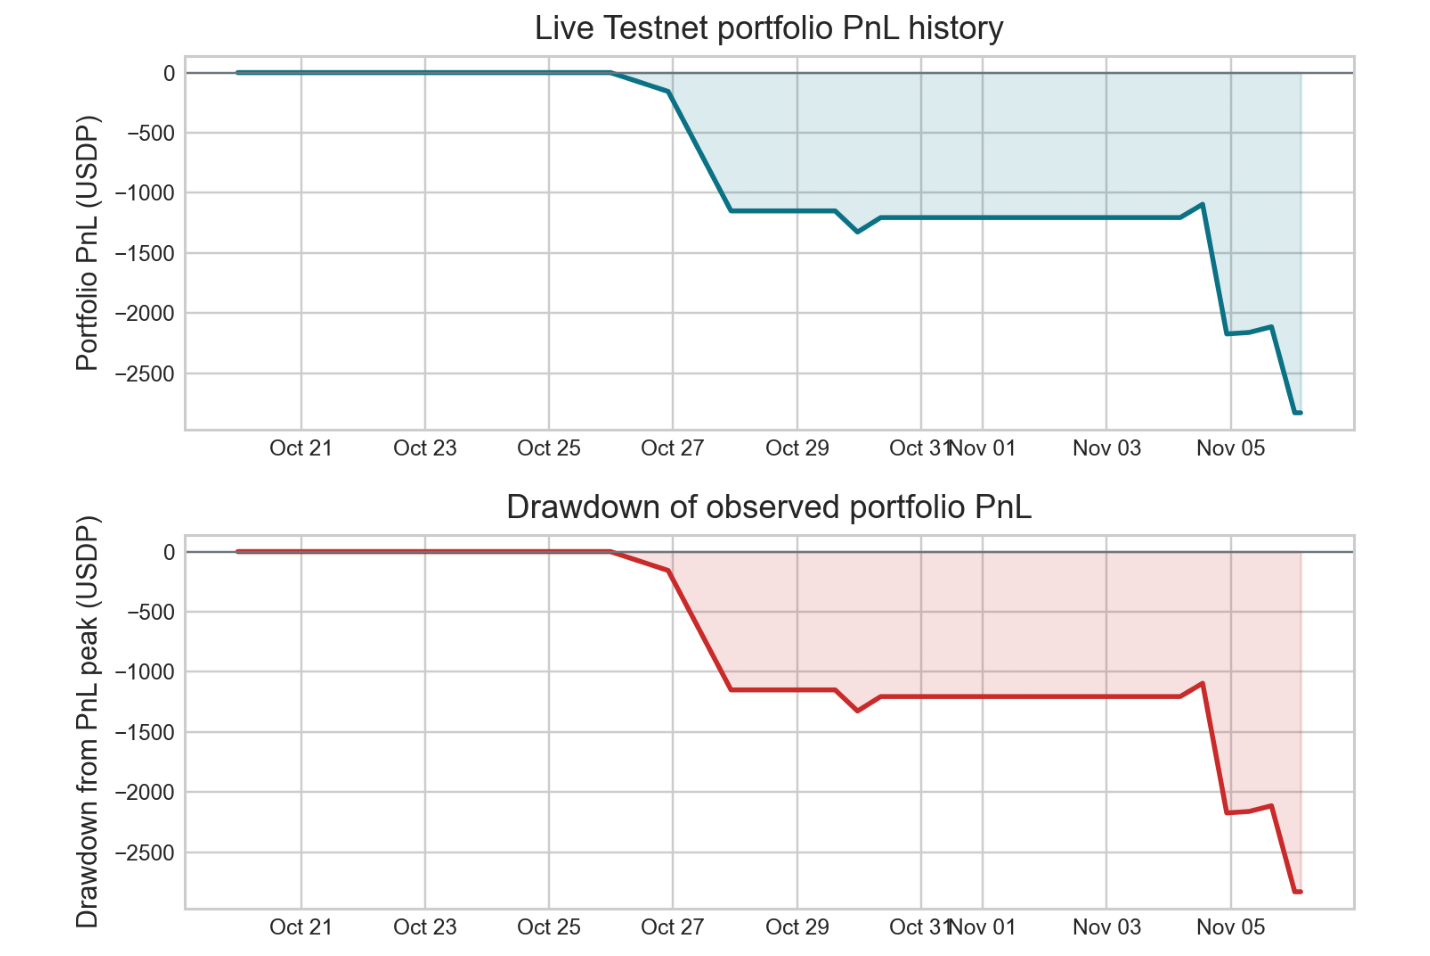
\includegraphics[width=.86\linewidth]{live_results.png}
\caption{Observed Testnet portfolio PnL (top) and drawdown from its PnL peak (bottom).}\label{fig:results}
\end{figure}

\section{Limitations and future work}
Correlation or beta can break during regime shifts; a residual can trend rather
than revert. Time exits are conservative operational bounds and require broader
walk-forward evidence. Historical tests use a simplified 28 bp pair round-trip
cost assumption; they do not fully reproduce market impact, latency, or adverse
liquidity. The small live sample does not justify recent-outcome tuning. Future
work should test beta-sized legs, explicit impact models, regime filters, and
longer walk-forward periods.

\section{Use of AI assistants}
An LLM-based coding assistant supported research prototyping, code drafting,
documentation, and debugging under human review. No LLM consumed live market
data or made trading decisions. Live signals and orders were generated by the
fixed deterministic rules described here.

\section{Open section}
We chose a transparent hourly rule and bounded exposure over faster or more
complex variants whose later-segment evidence was weaker after costs.

\appendix\section{Reproducibility checklist}
The code package contains configuration, execution and shadow runners, score
validation, dependencies, and a secret-free \texttt{.env.example}. It excludes
credentials, keys, runtime state, logs, and market-history files.
\begin{thebibliography}{9}\small
\bibitem{pa-rules} Perpetual Alpha 2026. \emph{Competition Rules, Scoring, and Technical Report Template}. Organizer materials, 2026.
\bibitem{hl-docs} Hyperliquid. \emph{API Documentation and Portfolio Graphs}. \url{https://hyperliquid.gitbook.io/hyperliquid-docs/}.
\end{thebibliography}\end{document}
